\documentclass[twoside]{article}
\input{ISC18-english.sty}
%%%%%%%%%%%%%%%%%%%%%%%%%%%%  Make sure to compile twice for proper cross-references. %%%%%%%%%%%%%%%%%%%%%%%
%%%%%%% For proper display of references, compile the document twice. %%%%%%%%%%%%%%%%%%%%% 
%%%%%%%%%%%%%%% If using TeX Live, compile using pdflatex command %%%%%%%%%%%%%%%%%%%%%%%
\usepackage{xcolor}
\usepackage[table]{xcolor}
\usepackage{soul}
\sethlcolor{yellow}
\begin{document}
\thispagestyle{empty}
%%%%%%%%%%%%%%%%% Article title header  %%%%%%%%%%%%%%%%%%%%
\fancyhead[LE]{DRL-AD Framework}
%%%%%%%%%%%%%%%%% Article authors header   %%%%%%%%%%%%%%%%%%%%
\fancyhead[RO]{Khadivi Noghredeh et al.}
\begin{center}
{
\includegraphics [height=25mm, width=150.3mm] {Images/isc18E}} \\
\vspace*{-1.8cm}
%\begin{center}
%\color{blue} 
%{\hspace{0.1cm}\rule{\textwidth}{1mm}}\\
%\end{center}
\vspace*{4cm}
%%%%%%%%%%%%%%%%% Article title  %%%%%%%%%%%%%%%%%%%%
{\Large \bf Intelligent Anomaly Detection with Deep Reinforcement Learning for Industrial Inspection}\\
%%%%%%%%%%%%%%%%% Article authors and affiliations %%%%%%%%%%%%%%%%%%%%
{\bf
	Amirhossein Khadivi Noghredeh$^1$ Abdollah Safari$^{1, }$\footnote[2]{{\bf Corresponding Author:} {\tt a.safari@ut.ac.ir }}, Fatemeh Ziaeetabar$^1$, Firoozeh Haghighi$^1$ \\
	$^1$School of Mathematics, Statistics and Computer Science, College of Science, University of Tehran, Tehran, Iran \\
}
\end{center}
\rule{\textwidth}{0.2mm}\\
%%%%%%%%%%%%%%%%% Article abstract  %%%%%%%%%%%%%%%%%%%%
\noindent{\bf Abstract:}\\
This work tackles pixel-level anomaly detection in industrial inspection with scarce defective data. We introduce a semi-supervised deep reinforcement learning framework enhancing detection via an adaptive neural batch sampler and robust autoencoder, balancing exploration and exploitation for subtle anomalies. MVTec AD evaluations show superior performance (AUC: 0.949 $\pm$ 0.03, $F1_{\max}$: 0.561 $\pm$ 0.20), showing favorable results compared to structurally comparable lightweight methods, and standard deviations confirm robustness despite the increased mean accuracy. This offers a scalable, statistically robust solution for manufacturing quality assurance.
 
\noindent{\bf Keywords:} 
Anomaly Detection, Reinforcement Learning, Outlier Detection, Computer Vision, Semi-Supervised Learning, Adaptive Batch Sampling \\
\noindent{\bf Mathematics Subject Classification (2010):} $68T07$, $68T45$, $62H30$. \\
\hspace{1cm}\rule{\textwidth}{0.2mm}\\
%%%%%%%%%%%%%%
\section{Introduction}

Industrial visual inspection plays a vital role in modern manufacturing, ensuring product quality, operational reliability, and brand reputation. The rapid growth of high-resolution imaging and automation has intensified the need for accurate anomaly detection systems \cite{bergmann2019improving}. Within this domain, pixel-level anomaly detection—identifying fine-grained defects such as scratches, contamination, or structural deformations—remains particularly critical. Yet, real-world deployment is challenging due to the scarcity of defective samples, the subtle and heterogeneous nature of anomalies, and the high cost of obtaining precise pixel-wise annotations \cite{bergmann2021mvtec} and \cite{pimentel2014}.

Existing strategies for anomaly localization span several learning paradigms, each with notable statistical constraints. Unsupervised reconstruction-based methods train solely on normal data, detecting anomalies through deviations from the learned manifold \cite{pimentel2014}. Classical solutions rely on autoencoders (AEs) \cite{baur2018} and variational autoencoders (VAEs) \cite{goodfellow2014}, with benchmarks such as MVTec AD promoting progress via perceptual loss formulations \cite{bergmann2019improving} and \cite{bergmann2021mvtec}. More advanced variants like VQ-VAE-2 \cite{yapp2024} improve latent representations but still face core challenges: overfitting to normal patterns, low sensitivity to subtle defects, and fixed thresholding strategies misaligned with image statistics. To address these issues, recent approaches integrate limited labeled anomalies, improving segmentation accuracy through semi-supervised learning \cite{kang2026} and \cite{chu2020}.

Generative models such as GANs \cite{goodfellow2014} and diffusion-based methods \cite{dai2025}, \cite{sun2025} and \cite{rombach2022} attempt to capture normal data distributions, identifying anomalies as samples that cannot be properly generated or embedded \cite{schlegl2017}. However, these pipelines often suffer from instability, mode collapse, or excessive computational cost, and may not surpass well-optimized reconstruction models in pixel-level accuracy \cite{bergmann2021mvtec}.

Fully supervised methods employing U-Net \cite{ronneberger2015}, DeepLab \cite{long2017}, or FCNs \cite{chen2018} achieve high accuracy when pixel-wise labels are abundant, such as in road crack detection \cite{shi2016} and \cite{chen2018}. However, industrial inspection rarely benefits from large annotated datasets due to the scarcity and annotation cost of defective samples \cite{ronneberger2015} and \cite{shi2016}. This limitation motivates semi-supervised learning (SSL), which combines the generalization of unsupervised frameworks with the precision of limited labeled data \cite{kang2026}.

Reinforcement learning has emerged as a promising mechanism for adaptive sample selection. The neural batch sampling (NBS) approach of \cite{chu2020} demonstrates the potential of RL-driven patch selection, yet suffers from constrained state representations, unstable periodic autoencoder resets, and reliance on historical loss profiles \cite{chu2020} and \cite{khadivi2025}. These limitations reduce robustness in dynamic industrial settings.

Extending our preliminary work \cite{khadivi2025}, which was confined to a set of limited scenarios, the present paper introduces major advancements: (1) a richer 6-channel state representation integrating structural priors; (2) replacement of unstable periodic resets with structured dropout, proven to reduce reward variance; (3) a simplified lightweight predictor operating directly on the residual error space; and (4) complete evaluation across all 15 MVTec AD classes with ablation and failure analysis. Consequently, this framework transforms adaptive sampling from a heuristic component into the core engine of a unified anomaly detection system, and achieves superior performance compared to VQ-VAE-2 \cite{yapp2024}, U-Net \cite{ronneberger2015}, and NBS-Reset \cite{chu2020}.

\section{Proposed Method}
We propose a semi-supervised deep reinforcement learning framework for pixel-level anomaly detection, consisting of three integrated modules: a DRL-guided neural batch sampler, a stable autoencoder (AE), and a lightweight predictor. Unlike prior work that relies on periodic AE resets causing reward instability \cite{chu2020}, we introduce structured dropout before the bottleneck, eliminating resets and reducing reward variance, which contributes to more stable training and ultimately more consistent final predictions. The overall workflow is illustrated in Figure \ref{fig:framework}.

\begin{figure}[ht]
	\begin{center}
		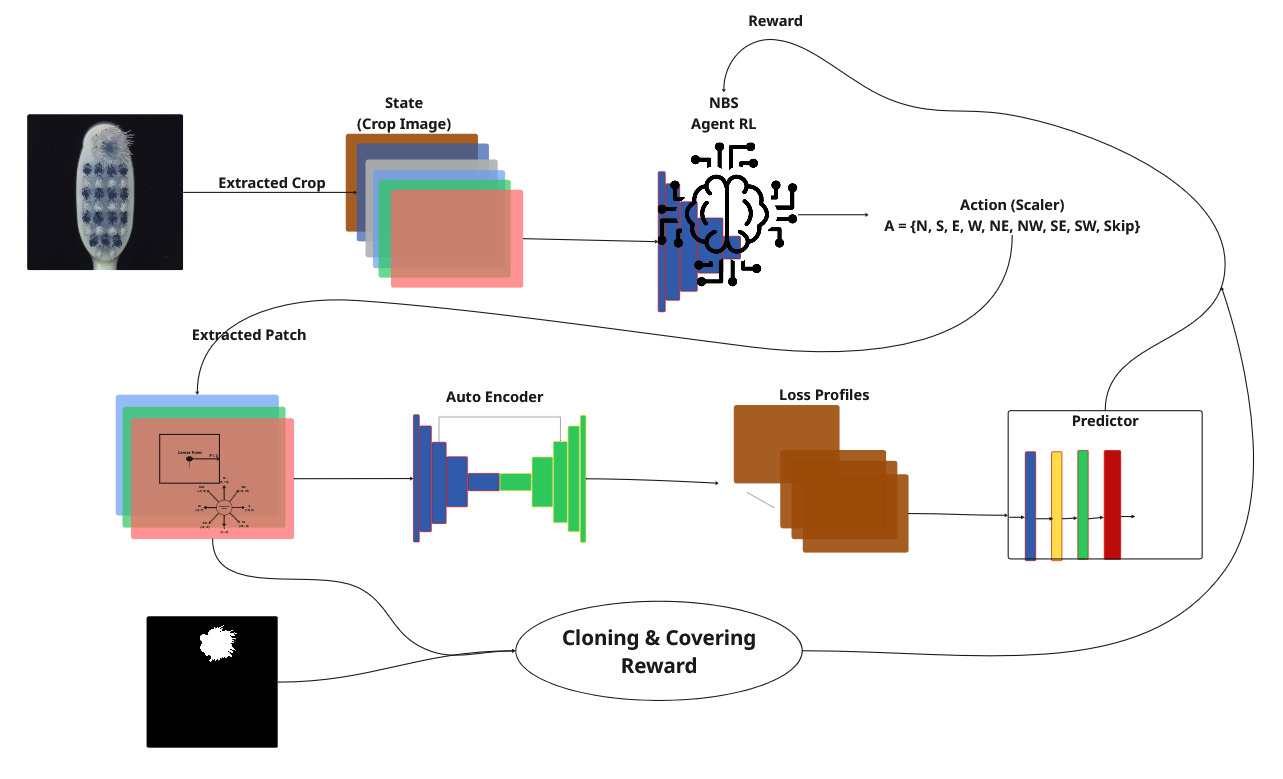
\includegraphics[width=12cm,height=6cm]{Images/detail_flowchart.jpg}
		\vspace{-0.2cm}
		\caption{\footnotesize{Architecture of the proposed DRL-based anomaly detection system.}}\label{fig:framework}
	\end{center}
\end{figure}

The framework operates as follows. For an input image \( I \in \mathbb{R}^{H\times W\times 3} \), we first construct a \textbf{6-channel state tensor} \( S(I) \) that guides the sampler. This tensor comprises: (1-3) original RGB channels; (4) a fused structural prior \( Z_{\text{fused}} = 0.7 Z_{\text{mae}} + 0.1 Z_{\text{var}} + 0.2 Z_{\text{grad}} \), where \( Z_{\text{mae}} \) is a pre-trained AE error map, \( Z_{\text{var}} \) is local intensity variance, and \( Z_{\text{grad}} \) is gradient magnitude; (5) a sampling history map \( H \) that penalizes revisited areas; and (6) the previous reconstruction error \( E_{t-1} \) for temporal consistency. The DRL agent \( \pi_\theta(a_t | s_t) \) navigates this state space with nine discrete actions (eight movement directions plus a SKIP action), extracting a batch of informative patches \( \mathcal{B} = \{P_1,\ldots,P_N\} \) from the image.

These patches serve as the training data for the autoencoder \( \text{AE}_\psi \). Critically, instead of resetting the AE periodically, we place a \textbf{dropout layer with rate \( p=0.3 \)} immediately before the bottleneck. During training, this injects controlled stochasticity, preventing overfitting and ensuring diverse reconstructions without abrupt parameter shocks. The AE is trained using mean squared error:
\[
\ell_{\text{MSE}} = \frac{1}{|\mathcal{B}|} \sum_{P\in \mathcal{B}} \| P - \text{AE}_\psi(P) \|_2^2.
\]
After each parameter update, the AE is applied in evaluation mode to all labeled anomalous images \( \{I_k^{\text{anomaly}}\} \) to generate residual error maps:
\[
\mathcal{E}_k = | I_k^{\text{anomaly}} - \text{AE}_\psi(I_k^{\text{anomaly}}) |.
\]

The predictor \( f_\phi \) is a lightweight fully convolutional network with dilated convolutions (rates 1,2,4,8) operating directly on the residual map \( \mathcal{E}_k \). It outputs a per-pixel anomaly probability \( \hat{Y} = f_\phi(\mathcal{E}_k) \) and is trained with a weighted binary cross-entropy loss that decays the normal-class weight from 1.0 to 0.15 over time, addressing class imbalance. The predictor's performance defines the primary learning signal for the sampler via a \textbf{composite reward}:
\[
R_t = \beta_t (R_{\text{clone}} + R_{\text{cover}}) + (1-\beta_t) R_{\text{pred}},
\]
where \( R_{\text{pred}} = -\ell_{\text{pred}} \) (negative segmentation loss), \( R_{\text{clone}} \) encourages selection of structurally rich patches (mean Sobel gradient), and \( R_{\text{cover}} = -\text{mean}(H_{P_t}) \) penalizes redundant sampling. The annealing factor \( \beta_t = \max(\beta_{\min}, 1 - \frac{t}{L}) \) shifts the agent from exploration (early training) to exploitation (late training).

The sampler's policy \( \pi_\theta \) is optimized via the REINFORCE algorithm to maximize expected cumulative reward. The gradient estimate is:
\[
\nabla_\theta J(\theta) \approx \frac{1}{T} \sum_{t=0}^{T-1} \left( \sum_{t'=t}^{T-1} R_{t'} \right) \nabla_\theta \log \pi_\theta(a_t | s_t).
\]

The training procedure follows a coordinated warm-up strategy. The autoencoder is first pre-trained on normal data to provide meaningful \( Z_{\text{fused}} \). The predictor is frozen for the first 50 iterations to allow the AE to generate stable error profiles, and policy updates begin after 100 iterations to avoid misleading reward signals. Once warm-up is complete, all three modules are updated jointly. At inference time, the sampler is deactivated; only the autoencoder and predictor run in a deterministic forward pass, enabling real-time deployment.

\section{Experimental Results}

\subsection{Experimental Setup}

We evaluate our proposed framework on MVTec AD \cite{bergmann2021mvtec} (15 categories, 5354 images). For each defect type, only 5 anomalous images with pixel-wise masks are used as labeled data. Inputs are resized to \(256\times256\times3\). Training uses Adam (lr=\(10^{-3}\), batch size 32), dropout rate \(p=0.3\), and 100 epochs per category on an NVIDIA RTX 3090 Ti GPU. Metrics are pixel-level AUC and \(F1_{\text{max}}\). Baselines include an unsupervised AE \cite{baur2018}, a supervised U-Net \cite{ronneberger2015}, VQ-VAE-2 \cite{yapp2024}, and NBS-Reset \cite{chu2020}. These baselines are not arbitrary; they were selected for their structural proximity to our framework to ensure a fair comparison, and each can be seen as an ablation study of our work.

\subsection{Results}
 
Table \ref{tab:combined} compares all 15 categories. Our method achieves mean AUC of 0.949 $\pm$ 0.03 and mean \(F1_{\text{max}}\) of 0.561 $\pm$ 0.20, outperforming all baselines. The standard deviations indicate that, despite the extent of increase in mean accuracy, our method maintains competitive robustness against the diversity of defect types.

The superior performance stems from three key factors: (i) the neural batch sampler (NBS) focuses reconstruction on informative local regions; (ii) replacing periodic resets with structured dropout reduces reward variance and stabilizes training; (iii) segmentation in the residual error space facilitates discriminative learning. The largest AUC gain occurs in Grid (+0.19), demonstrating the effectiveness of our approach in complex textures where NBS prevents overfitting to repetitive patterns. The improvement over supervised U-Net underscores the efficiency of DRL-guided active learning with scarce labels.

However, lower scores in Screw and Capsule reflect inherent limitations of patch-based reconstruction: micro-scale anomalies are attenuated by the autoencoder's bottleneck compression, while global structural deformations (e.g., in Transistor) lack sufficient residual contrast. Nevertheless, even in these challenging cases, our framework approximately localizes defects, which is often sufficient for industrial flagging. Qualitative results (Figure \ref{fig:results}) further confirm precise localization across diverse categories.

\begin{table}[h]
	\begin{center}
		\scriptsize
		\caption{Performance comparison on MVTec AD.}\label{tab:combined}
		\begin{tabular}{|l|c|c|c|c|c|c|c|}
			\hline
			Category & \multicolumn{2}{c|}{AUC} & \multicolumn{5}{c|}{\(F1_{\text{max}}\)} \\ \hline
			& VQ-VAE-2 & Ours & AE & U-Net & VQ-VAE-2 & NBS-Reset & Ours \\ \hline \hline
			Bottle & 0.84 & \textbf{0.98} & 0.34 & 0.31 & 0.39 & \textbf{0.80} & 0.76 \\
			Cable & 0.90 & \textbf{0.93} & 0.10 & 0.25 & \textbf{0.54} & 0.31 & 0.54 \\
			Capsule & 0.70 & \textbf{0.93} & 0.08 & 0.05 & \textbf{0.25} & 0.12 & 0.21 \\
			Hazelnut & 0.85 & \textbf{0.99} & 0.22 & 0.29 & 0.31 & 0.50 & \textbf{0.70} \\
			Metal Nut & 0.97 & 0.97 & 0.23 & 0.29 & 0.57 & 0.82 & \textbf{0.86} \\
			Pill & 0.79 & \textbf{0.99} & 0.09 & 0.14 & 0.58 & 0.42 & \textbf{0.77} \\
			Screw & 0.83 & \textbf{0.93} & 0.06 & 0.01 & \textbf{0.48} & 0.08 & 0.20 \\
			Toothbrush & 0.78 & \textbf{0.93} & 0.09 & 0.28 & 0.21 & \textbf{0.52} & 0.42 \\
			Transistor & \textbf{0.93} & 0.89 & 0.09 & 0.10 & 0.37 & 0.18 & \textbf{0.42} \\
			Zipper & 0.68 & \textbf{0.98} & 0.13 & 0.26 & 0.37 & \textbf{0.68} & \textbf{0.72} \\
			Carpet & 0.88 & \textbf{0.97} & 0.08 & 0.43 & 0.45 & \textbf{0.62} & \textbf{0.65} \\
			Grid & 0.83 & \textbf{0.92} & 0.02 & 0.12 & 0.19 & 0.17 & \textbf{0.32} \\
			Leather & 0.97 & 0.97 & 0.02 & 0.20 & 0.40 & 0.36 & \textbf{0.61} \\
			Tile & 0.86 & \textbf{0.95} & 0.21 & 0.37 & 0.40 & \textbf{0.64} & \textbf{0.71} \\
			Wood & 0.72 & \textbf{0.90} & 0.16 & 0.36 & 0.45 & \textbf{0.50} & \textbf{0.52} \\ \hline
			Mean & 0.835 $\pm$ 0.09 & \textbf{0.949} $\pm$ 0.03 & 0.128 $\pm$ 0.09 & 0.231 $\pm$ 0.12 & 0.397 $\pm$ 0.12 & 0.448 $\pm$ 0.23 & \textbf{0.561} $\pm$ 0.20 \\ \hline
		\end{tabular}
	\end{center}
\end{table}

\begin{figure}[ht]
	\begin{center}
		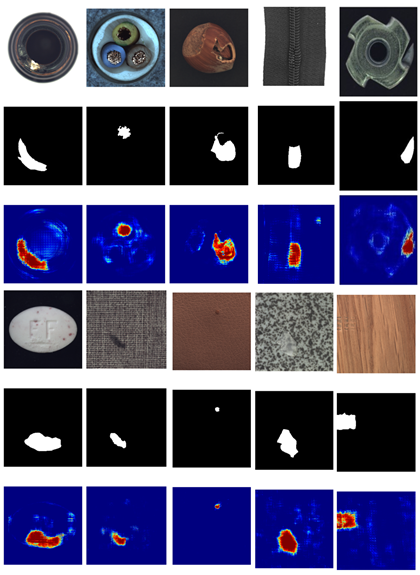
\includegraphics[width=10cm,height=12cm]{Images/qualitative_results.png}
		\vspace{-0.2cm}
		\caption{\footnotesize{Qualitative anomaly segmentation results on MVTec AD categories.}}\label{fig:results}
	\end{center}
\end{figure}

\section*{Discussion and Conclusion}   
We propose a DRL framework using structured dropout instead of periodic resets, achieving strong MVTec AD results (AUC 0.949, F1 0.561) and outperforming comparable lightweight methods. Our approach requires few annotations and runs fast; future work will explore Transformers and multi-scale strategies.

\begin{thebibliography}{9}
	
	\bibitem[Yapp and Doan (2024)]{yapp2024}
	Yapp A.K. and Doan N.C.N. (2024), Anomaly detection on MVTec AD using VQ-VAE-2, {\it Procedia CIRP}, 130, 1809-1814.
	
	\bibitem[Ronneberger et al. (2015)]{ronneberger2015}
	Ronneberger O., Fischer P. and Brox T. (2015), U-Net: Convolutional networks for biomedical image segmentation, {\it Proc. Int. Conf. Med. Image Comput. Comput.-Assist. Intervent. (MICCAI)}, 234-241.
	
	\bibitem[Pimentel et al. (2014)]{pimentel2014}
	Pimentel M.A.F., Clifton D.A., Clifton L. and Tarassenko L. (2014), A review of novelty detection, {\it Signal Process.}, 99, 215-249.
	
	\bibitem[Baur et al. (2018)]{baur2018}
	Baur C., Wiestler B., Albarqouni S. and Navab N. (2018), Deep autoencoding models for unsupervised anomaly segmentation in brain MR images, {\it Proc. Int. MICCAI Brainlesion Workshop}, 161-169.
	
	\bibitem[Bergmann et al. (2019a)]{bergmann2019improving}
	Bergmann P., L\"owe S., Fauser M., Sattlegger D. and Steger C. (2019), Improving unsupervised defect segmentation by applying structural similarity to autoencoders, {\it Proc. Int. Joint Conf. Comput. Vis., Imag. Comput. Graph. Theory Appl. (VISIGRAPP)}, 372-380.
	
	\bibitem[Bergmann et al. (2021)]{bergmann2021mvtec}
	Bergmann P., Batzner K., Fauser M., Sattlegger D. and Steger C. (2021), The MVTec anomaly detection dataset: A comprehensive real-world dataset for unsupervised anomaly detection, {\it Int. J. Comput. Vis.}, 129(4), 1038-1059.
	
	\bibitem[Goodfellow et al. (2014)]{goodfellow2014}
	Goodfellow I., Pouget-Abadie J., Mirza M., Xu B., Warde-Farley D., Ozair S., Courville A. and Bengio Y. (2014), Generative adversarial nets, {\it Proc. Adv. Neural Inf. Process. Syst. (NeurIPS)}, 2672-2680.
	
	\bibitem[Schlegl et al. (2017)]{schlegl2017}
	Schlegl T., Seeb\"ock P., Waldstein S.M., Schmidt-Erfurth U. and Langs G. (2017), Unsupervised anomaly detection with generative adversarial networks to guide marker discovery, {\it Proc. Inf. Process. Med. Imag. (IPMI)}, 146-157.
	
	\bibitem[Shi et al. (2016)]{shi2016}
	Shi Y., Cui L., Qi Z., Meng F. and Chen Z. (2016), Automatic road crack detection using random structured forests, {\it IEEE Trans. Intell. Transp. Syst.}, 17(12), 3434-3445.
	
	\bibitem[Chen et al. (2018)]{chen2018}
	Chen L.-C., Papandreou G., Kokkinos I., Murphy K. and Yuille A.L. (2018), DeepLab: Semantic image segmentation with deep convolutional nets, atrous convolution, and fully connected CRFs, {\it IEEE Trans. Pattern Anal. Mach. Intell.}, 40(4), 834-848.
	
	\bibitem[Long et al. (2017)]{long2017}
	Long J., Shelhamer E. and Darrell T. (2017), Fully convolutional networks for semantic segmentation, {\it IEEE Trans. Pattern Anal. Mach. Intell.}, 39(4), 640-651.
	
	\bibitem[Dai et al. (2025)]{dai2025}
	Dai Z., Zhang Y., Wang L., Chen X. and Liu H. (2025), SeaS: Few-shot industrial anomaly image generation with separation and sharing fine-tuning, {\it Proc. Int. Conf. Learn. Represent. (ICLR)}.
	
	\bibitem[Sun et al. (2025)]{sun2025}
	Sun H., Cao Y., Dong H. and Fink O. (2025), Unseen visual anomaly generation, {\it Proc. IEEE Conf. Comput. Vis. Pattern Recognit. (CVPR)}, 25508-25517.
	
	\bibitem[Rombach et al. (2022)]{rombach2022}
	Rombach R., Blattmann A., Lorenz D., Esser P. and Ommer B. (2022), High-resolution image synthesis with latent diffusion models, {\it Proc. IEEE Conf. Comput. Vis. Pattern Recognit. (CVPR)}, 10684-10695.
	
	\bibitem[Kang et al. (2026)]{kang2026}
	Kang B., Zhong Y., Deng L., Wang M. and Zhang J. (2026), Enhancing unsupervised unified anomaly detection via semi-supervised learning with multi-source uncertainty mining, {\it Neurocomputing}, 660.
	
	\bibitem[Chu and Kitani (2020)]{chu2020}
	Chu W.-H. and Kitani K.M. (2020), Neural batch sampling with reinforcement learning for semi-supervised anomaly detection, {\it Proc. Eur. Conf. Comput. Vis. (ECCV)}, 703-719.
	
	\bibitem[Khadivi Noghredeh et al. (2025)]{khadivi2025}
	Khadivi Noghredeh A., Safari A., Ziaeetabar F. and Haghighi F. (2025), DRL-Guided neural batch sampling for semi-supervised pixel-level anomaly detection, {\it arXiv preprint arXiv:2511.20270}.
	
\end{thebibliography}
 \end{document}